\chapter{La metodologia: dai Big Data all'analisi della capacità di un processo}
\label{chap:Big Data e l'analisi della capacità di un processo}

\section{Big Data}

Con la rapida diffusione della tecnologia dell'informazione, la maggior parte dei dati è diventata quasi totalmente disponibile in digitale. 
Sebbene i progressi dei sistemi informatici e delle tecnologie Internet abbiano visto lo sviluppo dell'hardware di calcolo, i problemi di gestione dei dati su larga scala esistono ancora adesso, nonostante stiamo entrando nell'era dei Big Data.  
\cite{tsai2015big}


I ``Big Data'' sono una grande quantità di dati strutturati e non strutturati che vengono raccolti, archiviati e analizzati per molti scopi, come obiettivi economici e di ricerca.  
\cite{techtarget}


I sistemi che elaborano e memorizzano i Big Data sono diventati una componente comune delle architetture di gestione dei dati nelle organizzazioni, insieme agli strumenti che supportano gli usi analitici dei Big Data. 
Oltre alla questione della dimensione dei dati, Doug  Lancy in una ricerca del 2001 ha presentato una definizione ben nota (chiamata anche 3V) per spiegare cosa sono: volume, velocità e varietà. 
La definizione di 3V implica, rispettivamente, che le dimensioni dei dati sono grandi, che i dati vengono creati rapidamente e che i dati esistono in più tipi e vengono acquisiti da fonti diverse:

\begin{itemize}
    \item il grande volume di dati in molti ambienti
    \item l'ampia varietà di tipi di dati spesso memorizzati nei sistemi di Big Data
    \item la velocità con cui molti dei dati vengono generati, raccolti ed elaborati.
\end{itemize}

Studi successivi hanno sottolineato che la definizione di 3V è insufficiente per spiegare i big data che abbiamo di fronte. Pertanto, per completare la spiegazione dei Big Data sono stati aggiunti veracità, validità, valore, variabilità, vocabolario e vaghezza. 
\cite{tsai2015big}


Con l'aumento delle capacità di archiviazione e la disponibilità di tecnologie avanzate di analisi dei dati, i Big Data stanno diventando sempre più importanti per le industrie manufatturiere.

Uno dei principali vantaggi dell'utilizzo dei Big Data nelle industrie è la possibilità di ottenere una maggiore efficienza nei processi produttivi. Ad esempio, i dati raccolti dalle macchine e dai sensori possono essere utilizzati per ottimizzare i parametri di produzione, ridurre i tempi di fermo macchina e migliorare la qualità del prodotto finale. Inoltre, l'analisi dei dati può aiutare a identificare eventuali problemi nei processi produttivi e a trovare soluzioni efficaci per risolverli.
\cite{Internet4things}


I big data possono anche essere utilizzati per prevedere la domanda del mercato e adattare la produzione di conseguenza, aumentando l'efficienza e riducendo gli sprechi.
Quindi, sono in grado anche di aiutare le industrie manufatturiere a sviluppare nuovi prodotti e servizi. Ad esempio, l'analisi dei dati dei clienti può fornire informazioni sui loro bisogni e preferenze, che possono essere utilizzate per sviluppare nuovi prodotti e servizi. Inoltre, l'analisi dei dati di mercato può aiutare le aziende a identificare nuove opportunità di business. 
\cite{o2015big}

Inoltre, i Big Data possono essere utilizzati per migliorare la sicurezza e la qualità dei prodotti. Ad esempio, l'analisi dei dati di qualità può aiutare a identificare problemi e a prevenire difetti nei prodotti. Inoltre, l'analisi dei dati di sicurezza può aiutare a identificare e prevenire rischi per la sicurezza sul posto di lavoro.
\cite{ThinkOpen}



Tuttavia, è importante notare che per trarre vantaggio dai Big Data, le aziende devono avere una solida strategia e un'adeguata infrastruttura tecnologica. Ciò significa che le aziende devono investire in tecnologie avanzate di raccolta, archiviazione e analisi dei dati, nonché formare il proprio personale per sfruttare al meglio queste tecnologie. Inoltre, le aziende devono essere in grado di gestire e proteggere i dati in modo sicuro, poiché i Big Data possono rappresentare anche un rischio per la sicurezza dei dati.
\cite{BigDataSecurity}



Con l'avvento dei Big Data è nata anche la Data Visualization.
La Data Visualization consiste nella rappresentazione grafica dei dati, in due o tre dimensioni, statica o dinamica. Ci sono molte tecnologie per la Data Visualization che utilizzano elementi visivi come mappe, grafici, barre, ecc. per fornire un modo semplice e intuitivo per visualizzare i dati. Questi strumenti sono utili per identificare situazioni anormali, tendenze o regolarità nei dati. I tool di Data Visualization sono fondamentali nell'industria perché forniscono un'interfaccia user-friendly che è vantaggiosa per la comunicazione tra gruppi operativi con competenze e conoscenze diverse. 
\cite{ScegliFornitore}


In sintesi, i Big Data stanno avendo un impatto significativo sulle industrie manufatturiere. Attraverso l'utilizzo di tecnologie avanzate di analisi dei dati, le aziende possono migliorare la qualità dei prodotti, aumentare l'efficienza e ridurre i costi, sviluppare nuovi prodotti e servizi, migliorare la sicurezza e la qualità dei prodotti, identificare nuove opportunità di business. Tuttavia, è importante notare che per trarre vantaggio dai Big Data, le aziende devono avere una solida strategia e un'adeguata infrastruttura tecnologica. 
\cite{o2015big}

%%%%%%%%%%%%%%%%%%%%%%%%%%%%%%%%%%%%%
\clearpage
\section{L'analisi di processo}
L'analisi di un processo è una metodologia statistica che punta a comprendere e analizzare le variabilità nella qualità di un processo produttivo. 
\cite{qualityi}


L'obiettivo dell'analisi di processo è quello di esaminare la stabilità dei processi attraverso i risultati emersi dagli indici di capacità di processo e valutare la robustezza del processo produttivo per le caratteristiche riportate del piano di controllo di qualità, tramite la definizione di un metodo standardizzato, accompagnato dalla frequenza di campionamento e dalla definizione dei requisiti minimi. 
\cite{blogkainexus}


Per stabilire un metodo standardizzato, è necessario specificare ex ante i metodi di controllo statistico di processo \textit{(Statistical Process Control)}.


Il Controllo Statistico di Processo, detto anche \textit{SPC} può essere descritto come l'utilizzo di una tecnica matematica o statistica che consente di mantenere i risultati di un processo entro specifici limiti, determinati attraverso l'analisi della variabilità intrinseca dei limiti di processo.
Questo sistema di controllo prevede di valutare la capacità del processo all'avvio e periodicamente, e di controllare il suo stato statistico, tramite l'utlizzo sistematico di \textit{Carte di Controllo} per definire, evidenziare e rimuovere eventuali cause che determinano la variabilità.
\cite{WikipediaSPC}


La rilevazione dello scarto quadratico medio, noto anche deviazione standard é uno dei principali metodi statistici applicabili. 
I limiti naturali della variazione di un processo si ricavano attraverso la correlazione tra la deviazione standard e la distribuzione normale.
Un processo viene poi suddiviso in due categorie, in base all'esito del'osservazione:
\begin{itemize}
\item sotto controllo statistico, ovvero quando il processo è influenzato unicamente da fattori casuali, non prevedibili
\item fuori controllo statistico, ovvero quando l'influenza delle variazioni del processo è causata da fattori specifici;
\end{itemize}

In particolare, se si prende in considerazione un processo sotto controllo statistico, effettuando un campionamento di dati, si può notare come il suo andamento temporale seguirà una distribuzione di frequenza che sarà molto simile a una distribuzione normale.


L'analisi del processo dal punto di vista della media e della sua variabilità è fondamentale per determinare i ``limiti naturali" del processo, entro i quali, se non accadono cause specifiche, il processo
manterrà il proprio andamento.
\cite{Joseph}


\begin{figure}[H]
  \centering
  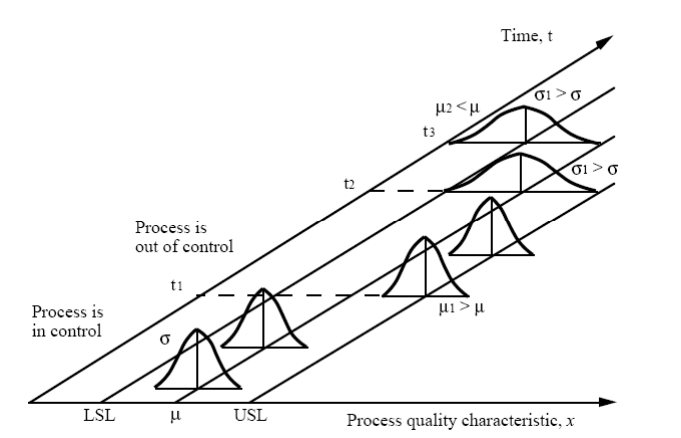
\includegraphics[width=0.75\textwidth]{img/process-quality-char.png}
  \caption{Caratteristiche di un processo statistico} 
  Fonte: Università di Roma, La Sapienza, Dipartimento di Ingegneria Meccanica e Aerospaziale, Programmazione e controllo della produzione, Teoria e metodi del controllo statistico di un processo produttivo
  \label{fig:process-quality-char.png}
\end{figure}

Dall'altra sponda, quando invece, questa distribuzione cambia, oppure variano i limiti, si può pensare ragionevolmente dal punto di vista statistico che stia agendo una ``possibile causa di fuori controllo''.

L'obiettivo, quindi, è quello di ridurre al massimo la variabilità, mantenere il processo sotto controllo, controllare le caratteristiche di qualità durante la produzione. 
\cite{qualityi}
\cite{ManagementAcademy}


%%%%%%%%%%%%%%%%%%%%%%%%%%%%%%%%%%%%%%%%%%%%%%%%%%%%%%%%%%%%%%%%%%%%%%%%%%%%%%%%%%%%%%%%%%%%
\section{Le cause di variabilità}
Per le cause di variabilità é possibile distinguere tra cause comuni o cause cosiddette speciali.
Le cause comuni (o normali), fanno parte del processo e riflettono il processo di variabilità naturale, insorgono casualmente durante il normale svolgimento del processo e ne determinano la fruttuazione naturale.

Tra le cause comuni è possibile identificare la variazione connaturata di materiali grezzi utilizzati nella linea produttiva, la mancanza di adeguata supervisione, i cambiamenti nelle condizioni lavorative e i malfunzionamenti delle macchine.
Bisogna notare che qualsiasi processo comprende delle cause comuni, ovvero un ammontare di ``variabilità naturale''. 

Tra le cause speciali, invece, si trovano le cause che determinano la variabilità non desiderata o anomala rispetto al naturale svolgimento del processo. 
Si tratta di fenomeni anomali che si presentano occasionalmente e possono essere rilevate monitorando continuamente il processo. 
\cite{reconsultsrl}

Le cause speciali possono essere attribuite, ad esempio, da particolari condizioni ambientali, dall'uso di un utensile sbagliato, dall'errore di un operatore o altro. 
Fin quando non verranno rilevate ed eliminate oppure corrette adeguatamente, esse continueranno ad influire in maniera imprevedibile sul processo, portandolo fuori controllo.

A tal fine, un processo sarà definito in base alla presenza o no delle cause speciali. Se in un processo vengono considerate solo la cause comuni di variabilità, eliminando tutte le cause speciali di variabilità: il processo sarà per definizione, ``sotto controllo statistico''.
\cite{qualityi}


\begin{figure}[h]
  \centering
  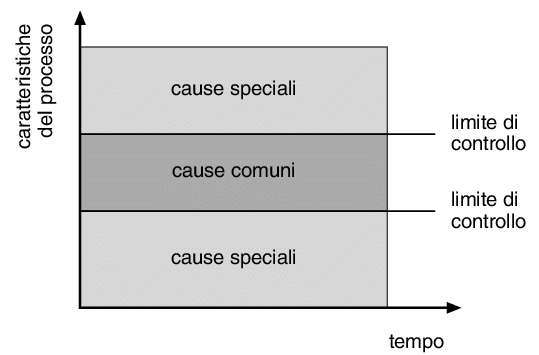
\includegraphics[width=0.75\textwidth]{img/cause.png}
  \caption{Posizione delle Cause di variabilità} 
  {Fonte: \url{https://www.researchgate.net/figure/Cause-comuni-speciali-e-limiti-di-controllo_fig5_289527561}
  Autore: Cristiano Fragassa, Marzo 2007}
  \label{fig:cause.png}
\end{figure}

D'altra parte, se un processo opera considerando anche la presenza della cause speciali, ovvero, fonti di variabilità che non fanno parte delle cause comuni, esso è per definizione, ``fuori controllo statistico''.


Il diagramma di Ishikawa, noto anche come diagramma a lisca di pesce o diagramma causa-effetto, è un ottimo strumento per visualizzare graficamente il potenziale delle cause speciali di uno specifico evento,
Le varia cause sono divise in macro categorie e individuano de percorsi che consentono di raggiungere un obiettivo finale che consiste, appunto, nell'effetto.
I gruppi di cause sono quattro fattori chiave \textit{le 4 M} che influenzano il processo produttivo,
a queste quattro cause fissate da Ishikawa se ne è aggiunta una quinta: l'ambiente, per cui si parla di \textit{5 M}.
\cite{ishi:book}

\begin{itemize}
  \item manodopera
  \item macchine (tecnologia, disponibilità)
  \item materiali (includono i materiali grezzi, consumabili e l'informazione)
  \item metodi (processi)
  \item misure (ispezione, ambiente);
  \end{itemize}


\begin{figure}[h]
  \centering
  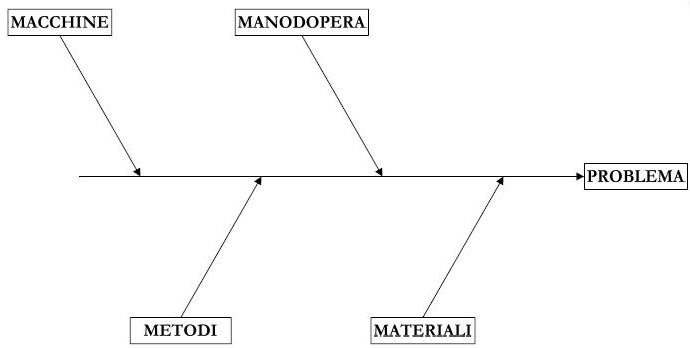
\includegraphics[width=0.75\textwidth]{img/ishikawa.png}
  \caption{Diagramma di Ishikawa} 
  {Fonte: \url{https://it.wikipedia.org/wiki/File:Diagramma_di_Ishikawa.jpg} 
  Autore: Marco Crescenzi, 2008} 
  \label{fig:ishikawa.png}
\end{figure}


In altri termini, si può dire che un processo è fuori controllo quando non segue un andamento casuale e la ragione può essere attribuita ad una delle \textit{5 M} di Ishikawa.

Due delle tecniche statistiche impiegabili nella metodologia SPC sono le carte di controllo e l'analisi della \textit{capability}.
\cite{HumanWare}

%%%%%%%%%%%%%%%%%%%%%%%%%%%%%%%%%%%%%%%%%%%%%%%%%%%%%%%%%%%%%%%%%%%%%%%%%
\section{La carta di controllo}
Molte caratteristiche possono essere espresse sotto forma di misurazione matematica. 

Una singola misura di una caratteristica di qualità, come possono essere, la dimensione, il peso o il volume, viene chiamata variabile.
A tal proposito nasce la Carta di controllo, ovvero, uno strumento utilizzato nell'ambito della statistica per mantenere sotto controllo i vari parametri di un processo. 
\cite{montgomery2009statistical}

La carta di controllo è uno strumento utile anche per monitorare l'evoluzione del processo e capire se un processo e sotto-controllo oppure fuori controllo (presenza o no delle cause speciali).

Se un processo è fuori controllo, la carta di controllo, da un'ipotetica indicazione del motivo del fuori controllo.
Fondamentalmente è una rappresentazione grafica di un processo nel tempo.

Per elaborare una carta di controllo è necessario compiere delle operazioni per un certo numero di campioni, ricavando parametri statistici come media, deviazione standard, range. 

Esistono due macro categorie per le carte di controllo, in base al tipo di dati estrapolati dall'analisi del processo in esame e sui quali sono costruite. 
Vi sono le carte per variabili, utilizzate nel caso di variabili quantitative continue oppure le carte per attribuiti, utilizzate nel caso di variabili quantitative discrete. 
\cite{DiNardo}


Qualora ci si ritrovi a lavorare con una caratteristica di qualità, che è una variabile, sarà necessario monitorare il valore medio della caratteristica e la sua variabilità.
Il controllo del processo in media oppure della qualità della media del processo, tendenzialmente viene fatto tramite la carta di controllo per valori medi. 


Dal lato opposto, la variabilità di processo può essere monitorata o con una carta di controllo per la deviazione standard, detta anche \textit{S control chart} oppure qualora il numero di valori che costituisce la misura è troppo piccolo, affinché la deviazione standard del campione sia statisticamente attendibile viene utilizzata la carta di controllo range, detta anche \textit{R control chart}.
\cite{montgomery2009statistical}


I limiti inferiori e superiori sono calcolati in base ad una distribuzione di frequenza teorica che cambia in funzione del tipo di dati che vengono analizzati, può essere quindi una distribuzione Gaussiana, una Poisson, una binomiale, una T di Student.
Tendenzialmente si utilizza una distribuzione Gaussiana. 
La distribuzione gaussiana, nota anche come distribuzione normale o di Gauss, è una distribuzione di probabilità continuamente utilizzata in molte aree della matematica e della scienza. La sua forma è caratterizzata da una curva a campana simmetrica intorno alla media (o alla mediana), con la maggior parte dei valori concentrati intorno al valore centrale e meno valori estremi. La distribuzione gaussiana è descritta dalla sua media (o mediana) e la sua deviazione standard. La funzione di densità di probabilità per la distribuzione normale è nota come ``funzione gaussiana'' o ``curva normale''.
\cite{WikipediaGauss}



L'attribuzione dei limiti generalmente viene fatta nel modo seguente:

I limiti di controllo sono guidati dalle cause comuni (interne) di variabilità del processo. 
Supponendo che \textit{w} sia un campione statistico che misuri alcune caratteristiche di interesse e supponendo che la media di \textit{w} sia $\mathit{\mu_w}$ e la deviazione standard di \textit{w} sia $\mathit{\sigma_w}$. 

Allora la linea centrale, detta anche \textit{CL: Central Line} che rappresenta la media del processo in controllo, \textit{UCL: Upper Control Limit} che rappresenta il limite superiore di controllo e \textit{LCL: Lower Control Limit}, ovvero il limite inferiore di controllo
si riuniscono nella formazione dei i limiti entro i quali un processo può essere definito in controllo, saranno:


\begin{equation}
  \begin{cases}
  UCL = \mu_w + L\sigma_w\\
  CL = \mu_w\\
  LCL = \mu_w - L\sigma_w \\
\end{cases}
\label {eqn: CONTROL LIMITS}
\end{equation}


Dove \textit{L} è la ``distanza'' riferita ai limiti di controllo, dalla linea centrale \textit{CL}, espressa in termini di scarto quadratico dalla media.
Questo enunciato, è un approccio generale per decidere i limiti di controllo, tuttavia esistono delle specifiche formule che vanno applicate in base alla dimensione del campione e al campo di applicazione.

Una volta definiti i limiti di controllo e osservando la distribuzione del campione di riferimento, sarà possibile individuare eventuali andamenti sistematici dei valori che rappresentano l'evoluzione del processo nel tempo. 

Da qui in poi, saranno poi finalmente visibili andamenti anomali che potranno essere identificabili ad alcune le cause che lo hanno provocato, ad esempio, un andamento ciclico crescente o decrescente della caratteristica misurata, o altri tipi di andamento, trends che rilevano determinate condizioni da correggere, seppur quando le misure restino entro i limiti.

Il processo verrà definito fuori controllo, qualora uno o più punto cadono fuori dai limiti di controllo. 
A tal proposito verranno analizzati i punti che cadono fuori dai limiti di controllo, e verranno adottate delle misure correttive. 
\cite{montgomery2009statistical}


La Carta di Controllo rende possibile comprendere se un processo è fuori controllo (co-presenza di cause speciali) e rilevare eventuali cause speciali di variazione. 
Tuttavia non vengono usate con lo scopo di definire informazioni sulla conformità del processo con limiti di specifica.
L'utilizzo della carta di controllo non è sufficiente a comprendere la reale capacità di un processo nè come questo possa essere migliorato.

In generale, la carta di controllo prende questa forma:
%%% grafico control chart
\begin{figure}[h]
  \centering
  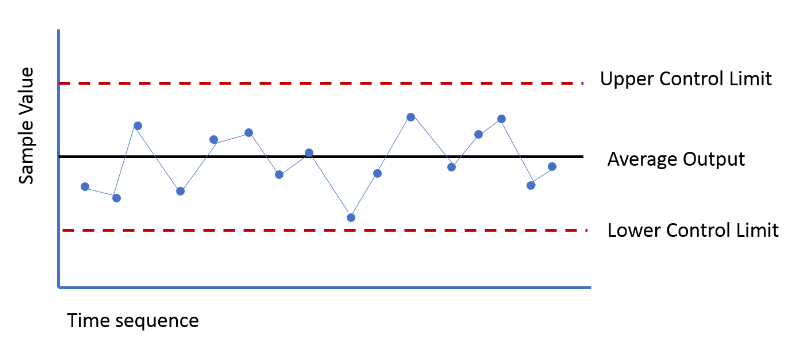
\includegraphics[width=0.85\textwidth]{img/controlchart.png}
  \caption{Carta di controllo con evidenza dei propri UCL/LCL} 
  {Fonte: \url{https://www.zerounoweb.it/analytics/balanced-scorecard-bsc-dinamiche-per-una-data-visualization-mulitimensionale/} Autore: Luigi Buglione}
  \label{fig:controlchart.png}
\end{figure}


Talvolta, possono interessare cose come, le tolleranze di lavorazione o altre specifiche di output del processo. 

La capacità di processo \textit{(process capability)} è una metodologia che, in riferimento ad una determinata attività, operazione, fase o processo caratterizzato da ripetività, consente di valutare quanto un processo produttivo, possa soddisfare una specifica di produzione o specifiche espresse dal cliente in termini di target e di limiti di specifica.
Con lo scopo finale di definire, analizzare e verificare le condizioni che determinano la variabilità dell'oggetto in analisi.
L'essenziale motivo per il quale la capacità di processo è preferibile rispetto ad altre tecniche, viene dal fatto che essa ci permette di valutare, monitorando, due aspetti caratteristici del processo:
\begin{itemize}
  \item la dispersione del processo
  \item la centratura del processo;
  \end{itemize}


Un processo con eccessiva variabilità è distinguibile dal fatto che, un'ampia porzione di area è al di fuori dei limiti di specificazione, nelle due direzioni.
Qualora non vi sia una variabilità elevata, è possibile rilevare un numero di dati esterni ai limiti se il processo non è centrato rispetto al valore di target. 
\cite{UniRoma}




\section{Gli indici di capacità di processo}
Lo studio della capacità di processo è eseguito mediante il calcolo di alcuni indicatori chiave: indice di potenzialità del processo e di prestazione del processo. 
Qualora si abbia a che fare a che fare con un processo stabile (verificato con una quantità di dati indipendenti), la cui variabilità è dovuta solo ed esclusivamente alle cause comuni di variabilità, gli indici utilizzati sono il \textit{Process Capability}, detto anche $CP$ e il \textit{Process Capability Index}, detto anche $CPK$, ovvero indici di potenzialità del processo. 


D'altra parte, qualora i processi con cui si abbia a che fare, abbiano informazioni limitate tali da non poterne ancora definire la stabilità, il $CP$ e il  $CPK$ saranno omessi in funzione di altri due indici, detti $PP$: \textit{Process Perfomance} e il $PPK$: \textit{Process Perfomance Index}, ovvero inidici di prestazione del processo.
In questo caso, non si parla di analisi della capacità di processo ma della capacità di prestazione.
\cite{Meetheskilles}


Con potenzialità del processo ci riferiamo in particolare alla capacità potenziale del processo a mantenere una determinata caratteristica in modo costante all'interno dei limiti di specifica prefissati.

\begin{itemize}
  \item l'indice di potenzialità del processo $CP$, valuta la prestazione quantitativa rapportando l'ampiezza della tolleranza prescritta e l'ampiezza della dispersione del processo.
La variabilità totale è detta anche tolleranza naturale del processo ed è rapportata dal valore $\mathit{6\sigma}$. 

% CP 
L'indice $CP$ è definito come: 
\begin{equation}CP =\frac{UTL-LTL}{6\sigma} 
\label {eqn: CP}
\end{equation}

dove $UTL$ ed $LTL$ sono rispettivamente i limiti di tolleranza superiorori ed inferiori di specifica dati dal piano di controllo e $\mathit{\sigma}$ la deviazione standard del processo calcolata su un numero contenuto di dati (tra 30 e 50).


Il $CP$ è dunque la misura del rapporto tra le dispersione ammissibile per il processo, calcolata dalla differenza tra i limiti di tolleranza, e la dispersione reale, rappresentata da sei volte la deviazione standard, detta anche tolleranza naturale. 
Quindi all'aumentare del valore della deviazione standard, il $CP$ diminuisce.
Questo vuol dire che processi con cause comuni di variazioni molto piccole hanno un elevato valore di $CP$.
\cite{WikCP}



Per una distribuzione normale, l'intervallo compreso tra i due estremi $\mathit{\pm3\sigma}$ include il 99,73\% dei valori di $X$ e, in corrispondenza, si ha il 0,27\% di valori esterni.
Di conseguenza, se l'intervallo di specificazione è maggiore di $\mathit{6\sigma}$ (ovvero se l'indice $CP$ è maggiore di 1) significa, che mediamente si producono meno del 2,7\% di pezzi non conformi e cioè che il processo può ritenersi capace.
Il valore target $CP$ tuttavia, è fissato in base a requisiti specifici di procedure interne, il processo sarà definibile capace qualora il $CP$ è maggiore del target prefissato.
\cite{montgomery2009statistical}

Valori di $CP$ superiori a 1,33 indicano che il processo è adeguato per soddisfare le specifiche. Valori di $CP$  compresi tra 1,33 e 1,00 indicano che il processo processo è adeguato a soddisfare le specifiche ma richiedono uno stretto controllo.
 Valori di $CP$ inferiori a 1,00 indicano che il processo non è in grado di soddisfare le specifiche. Se il processo è centrato all'interno delle specifiche e approssimativamente "normale", allora $CP$ = 1,00 risulta in una frazione non conforme dello 0.27\%. 
 Tale valore è noto anche come potenziale di processo. 
 \cite{Wooluru}
 


L'indice $CP$ è un indicatore efficace della capacità di processo, ma non è sufficiente da solo. 
Il $CP$ controlla solo la dispersione del processo, ma non fornisce informazioni sulla sua centratura. 
Un alto valore di $CP$, che dovrebbe indicare un processo capace, potrebbe in realtà produrre un alto numero di scarti a causa della deriva della media del processo verso i limiti di tolleranza.
Per far fronte a questo problema si introduce l'indice $CPK$.
\cite{qualityi}

\item l'indice di prestazione del processo $CPK$, a differenza del $CP$, considera anche la posizione del processo rispetto ai limiti di tolleranza. Esso considerando anche la centratura del processo, valuta la capacità effettiva di un processo di mantenere una determinata caratteristica in modo costante all'interno dei limiti di specifica prefissati.
Viene calcolato come il minimo tra la distanza del valore medio del processo dal limite di tolleranza superiore rapportato al semintervallo di dispersione e la distanza tra il valore medio dal limite di tolleranza inferiore, rapportato alla stessa quantità. 
\cite{SixSigma}


\begin{equation}CPK = min\left(\frac{UTL-\bar{X}}{3\sigma} ; 
\frac{\bar{X}-LTL}{3\sigma}\right)
\label {eqn: CPK}
\end{equation}

Scegliendo il minore dei due valori a destra e sinistra rispetto al valore medio, è possibile determinare quando il processo è capace sul lato peggiore, ovvero quello rappresentato dalla coda della Gaussiana più vicina al limite di tolleranza. 
\end{itemize}

\begin{itemize}
\item se $CPK$ è negativo, allora quasi la totalità dei pezzi sono fuori tolleranza
\item se $CPK$ è uguale 0, allora la metà dei pezzi prodotti sono fuori tolleranza
\item se $CPK$ è compreso tra -1 e 0, allora più della metà dei pezzi prodotti sono fuori tolleranza
\item se $CPK$ è uguale a 1, si è sul limite della lavorazione di pezzi non buoni
\item se $CPK$ è compreso tra 0 e 1, allora una parte dei pezzi prodotti del processo cadono oltre i limiti
\item se $CPK$ è maggiore di 1, l'ampiezza $\mathit{6\sigma}$ dei pezzi prodotti cade completamente nei limiti di tolleranza, si ha un buon mezzo di lavorazione;
\end{itemize}
\cite{qualityi}


Se l'indice $CP$ risulta uguale all'indice $CPK$ allora il processo è situato esattamente al centro dei limiti delle specifiche.
D'altra parte invece se l'indice $CP$ è diverso dall'indice $CPK$ allora il processo non è sufficiente ed è necessario selezionare un nuovo parametro di processo. 
\cite{yunus2016preliminary}


Gli indici in questione sono preferiti rispetto ad altri metodi statistici e tale motivo è imputabile alla possibilità di riassumere in modo molto coinciso i dati di un processo produttivo, con il vantaggio, di essere facilmente interpretabiili e paragonabili tra loro.
Pertanto, la comodità di tali indici si rende utile per confrontare le capacità di processo relative a differenti tipi di processi. 
\cite{Meetheskilles}

% \begin{figure}[h]
%   \centering
%   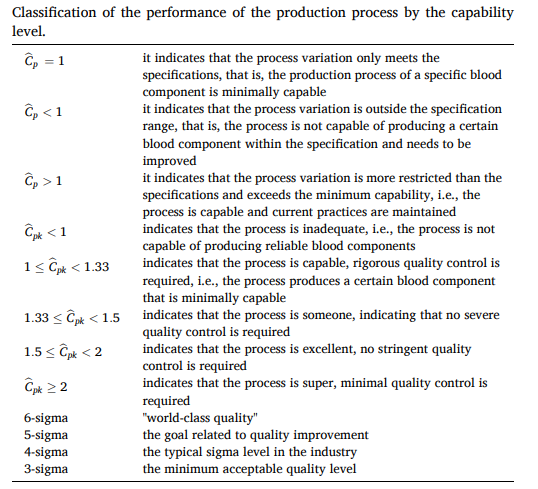
\includegraphics[width=0.85\textwidth]{img/cp-cpk-classification.png}
%   \caption{Classificazione degli indici di capacità di processo} 
%   {Fonte: Process capability indexes: Trends and developments in the manufacturing 
% of blood components, Autore: Paulo Pereira}
%   \label{fig:cp-cpk-classification.png}
% \end{figure}
